\subsection{Visual Studio Code}

Based on the book by April \cite{speight_2020}.

\begin{figure}[H]
\centering
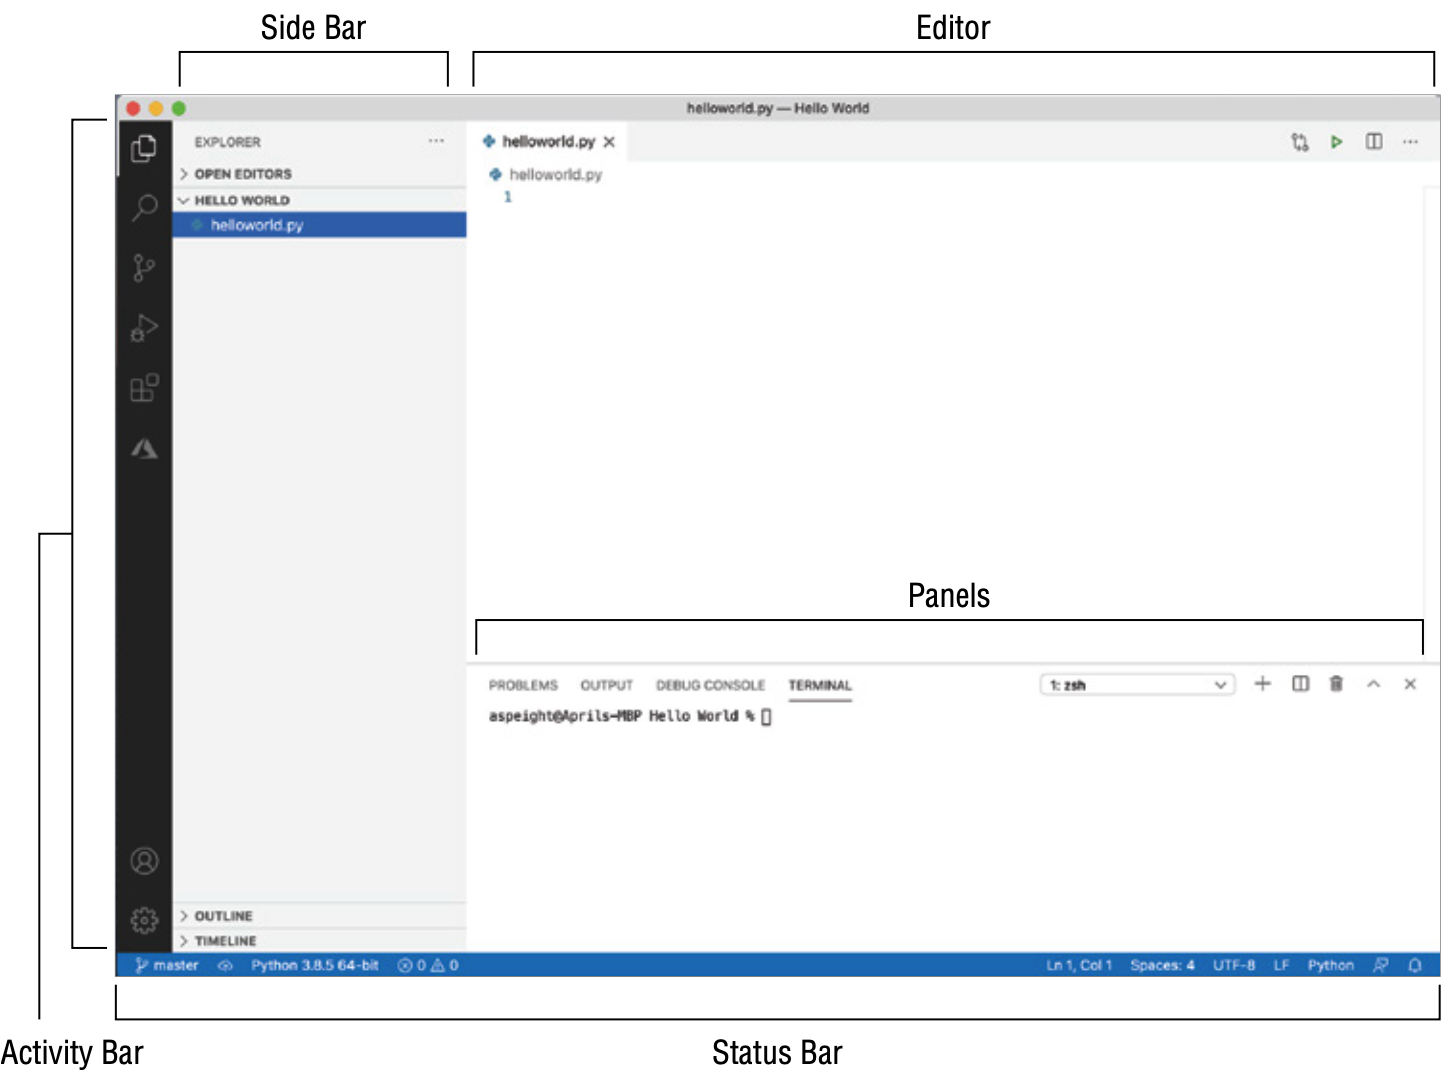
\includegraphics[scale=0.4]{appendix/vscode/vscodeui}
\caption{The visual studio code interface.}
\end{figure}

Activity bar on the far-left side allows switching between views, with quick access to tasks such as:
\begin{enumerate}[label=\roman*.]
\setlength{\itemsep}{0pt}
\item Explorer: file and folder management
\item Search: global search and replace, can use plain text or regex
\item Source Control: Git source control
\item Run: for debugging, such as variables, call stacks, breakpoints
\item Extensions: browsing, installation, management of extensions
\end{enumerate}
Activity bar may also provide custom views from extensions installed from Extension Marketplace. Views may be hidden, dragged and dropped around.\\

Side bar displays active view. Editor where files may be edited, may be resized, and top editor region changes depending on the type of file active in the editor; the top bar may also have a Source Control view if project is connected to git; files may be pinned and grouped by tabs.

\begin{figure}[H]
\centering

\includegraphics[scale=0.4]{appendix/vscode/makechanges}
\caption{Source control button}
\end{figure}

Panels are for debugging information, errors and warnings; and also for opening an integrated terminal on the root of the project. A REPL terminal (Python standard shell) may also be opened.\\

The status bar contains information about the opened project and files being edited. This includes: source control management with Git, total number of problems for the opened programs, line/column, indentation settings for space or tabs, encoding setting, end-of-line sequence setting, language mode, VS Code feedback mechanism, and notifications.\\

The command palette at the very top of the UI can be used to run commands to execute editor tasks in addition to extension commands.\\

\subsubsection{Setting Up Python}

To set default interpreter path in VS Code, in settings editor, search for \hlt{python.pythonPath}. In Python: Default Interpreter Path setting, enter the path to the interpreter.\\

To enable Quick Fix which help fix issues identified by warnings or errors (with lightbulb popping up), in settings editor, search for \hlt{python.jediEnabled}, then set it to false.\\

IntelliSense is a variety of tools to assist wth programming, such as code completion, object definition, location of object or variable declarations. These are triggered by either pressing Ctrl+Spacebar, or by tying a trigger character (i.e., a dot character in Python).\\

If linter detects any errors, these will be present in the Panels' Problem tab.\\

Refactoring is used to maintain functionality while improving the internal structure or architecture of a program. This should be a routine task that occurs before any updates or new features are added to a program. VS Code can help with refactoring via the following commands in Command Palette: Extract Variable, Extract Method, Sort Imports. Refactoring requires the \hlt{Rope} library.\\
Extract variable command allows extracting all similar occurrences of the same constant value of expression in multiple places, and replaces it with a variable. May be accessed via Python Refactor: Extract Variable.\\
Extract method command extracts all similar occurrences of selected expression or block, creates a new method, and replaces the expression with a method call. May be accessed via Python Refactor: Extract Method.\\
Sort imports method uses \hlt{isort} packages to consolidate specific imports from the same module into a single import statement, and organises 'import' statements in alphabetical order.\\

If a code pattern is repeated within a file or across multiple files, code snippets may be used, by searching in Command Palette for Snippets: Configure User Snippets. 